\DiaryEntry{Max-Flow Algorithms, Further Applications}{2020-06-26}{Algorithms}

\subsection{Other Flow Networks}

In the beginning we defined flow networks as having one source $s$ and one sink $t$ only. In addition, we did not allow for anti-parallel edges between two vertices. Here we show how we can get around these restrictions.

The left Figure below shows a network with several sources and sinks. We can solve this problem by introducing two new vertices, a ``super-source'' $s$, and a ``super-sink''$t$ as shown in the right Figure. The super-source $s$ is connected to the existing sources ($s_1 \ldots s_5$) via edges having infinite capacities; the super-sink is connected to the existing sinks ($t_1 \ldots t_3$) via edges having infinite capacities. We can now solve the maximum-flow problem with any algorithm on this extended flow network.

\begin{figure}[H]
\centering
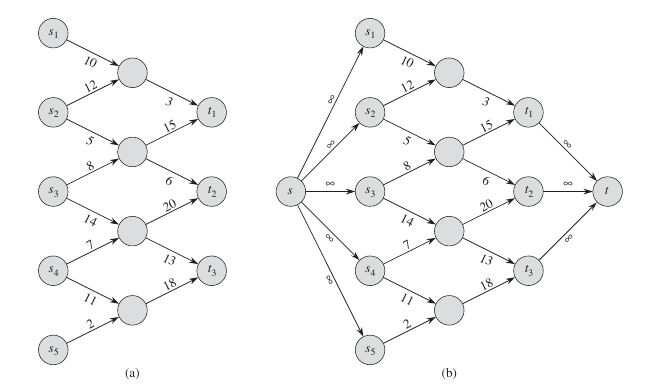
\includegraphics[scale=0.65]{images/max_flow_04_01.png}
\end{figure}

In case of anti-parallel edges, we can introduce an additional vertex which transports one of the flows. The following Figure illustrates the principle. On the left we have two anti-parallel edges between vertices $v_1$ and $v_2$. We extend the flow network by vertex $v'$ as shown on the right: The edge $v_1 \rightarrow v_2$ with capacity $10$ is replaced by the path $v_1 \rightarrow v' \rightarrow v_2$ (each edge having capacity $10$); the edge $v_2 \rightarrow v_1$ with capacity $4$ is not changed. The resulting network is again a flow network and can be solved by max-flow algorithms.

\begin{figure}[H]
\centering
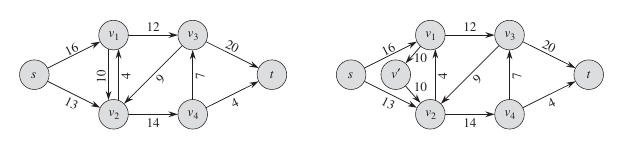
\includegraphics[scale=0.65]{images/max_flow_04_02.png}
\end{figure}



%%% Local Variables:
%%% mode: latex
%%% TeX-master: "journal"
%%% End:
